\section{Konzept 2: Druckluft}
\begin{figure}[h!]
	\centering
	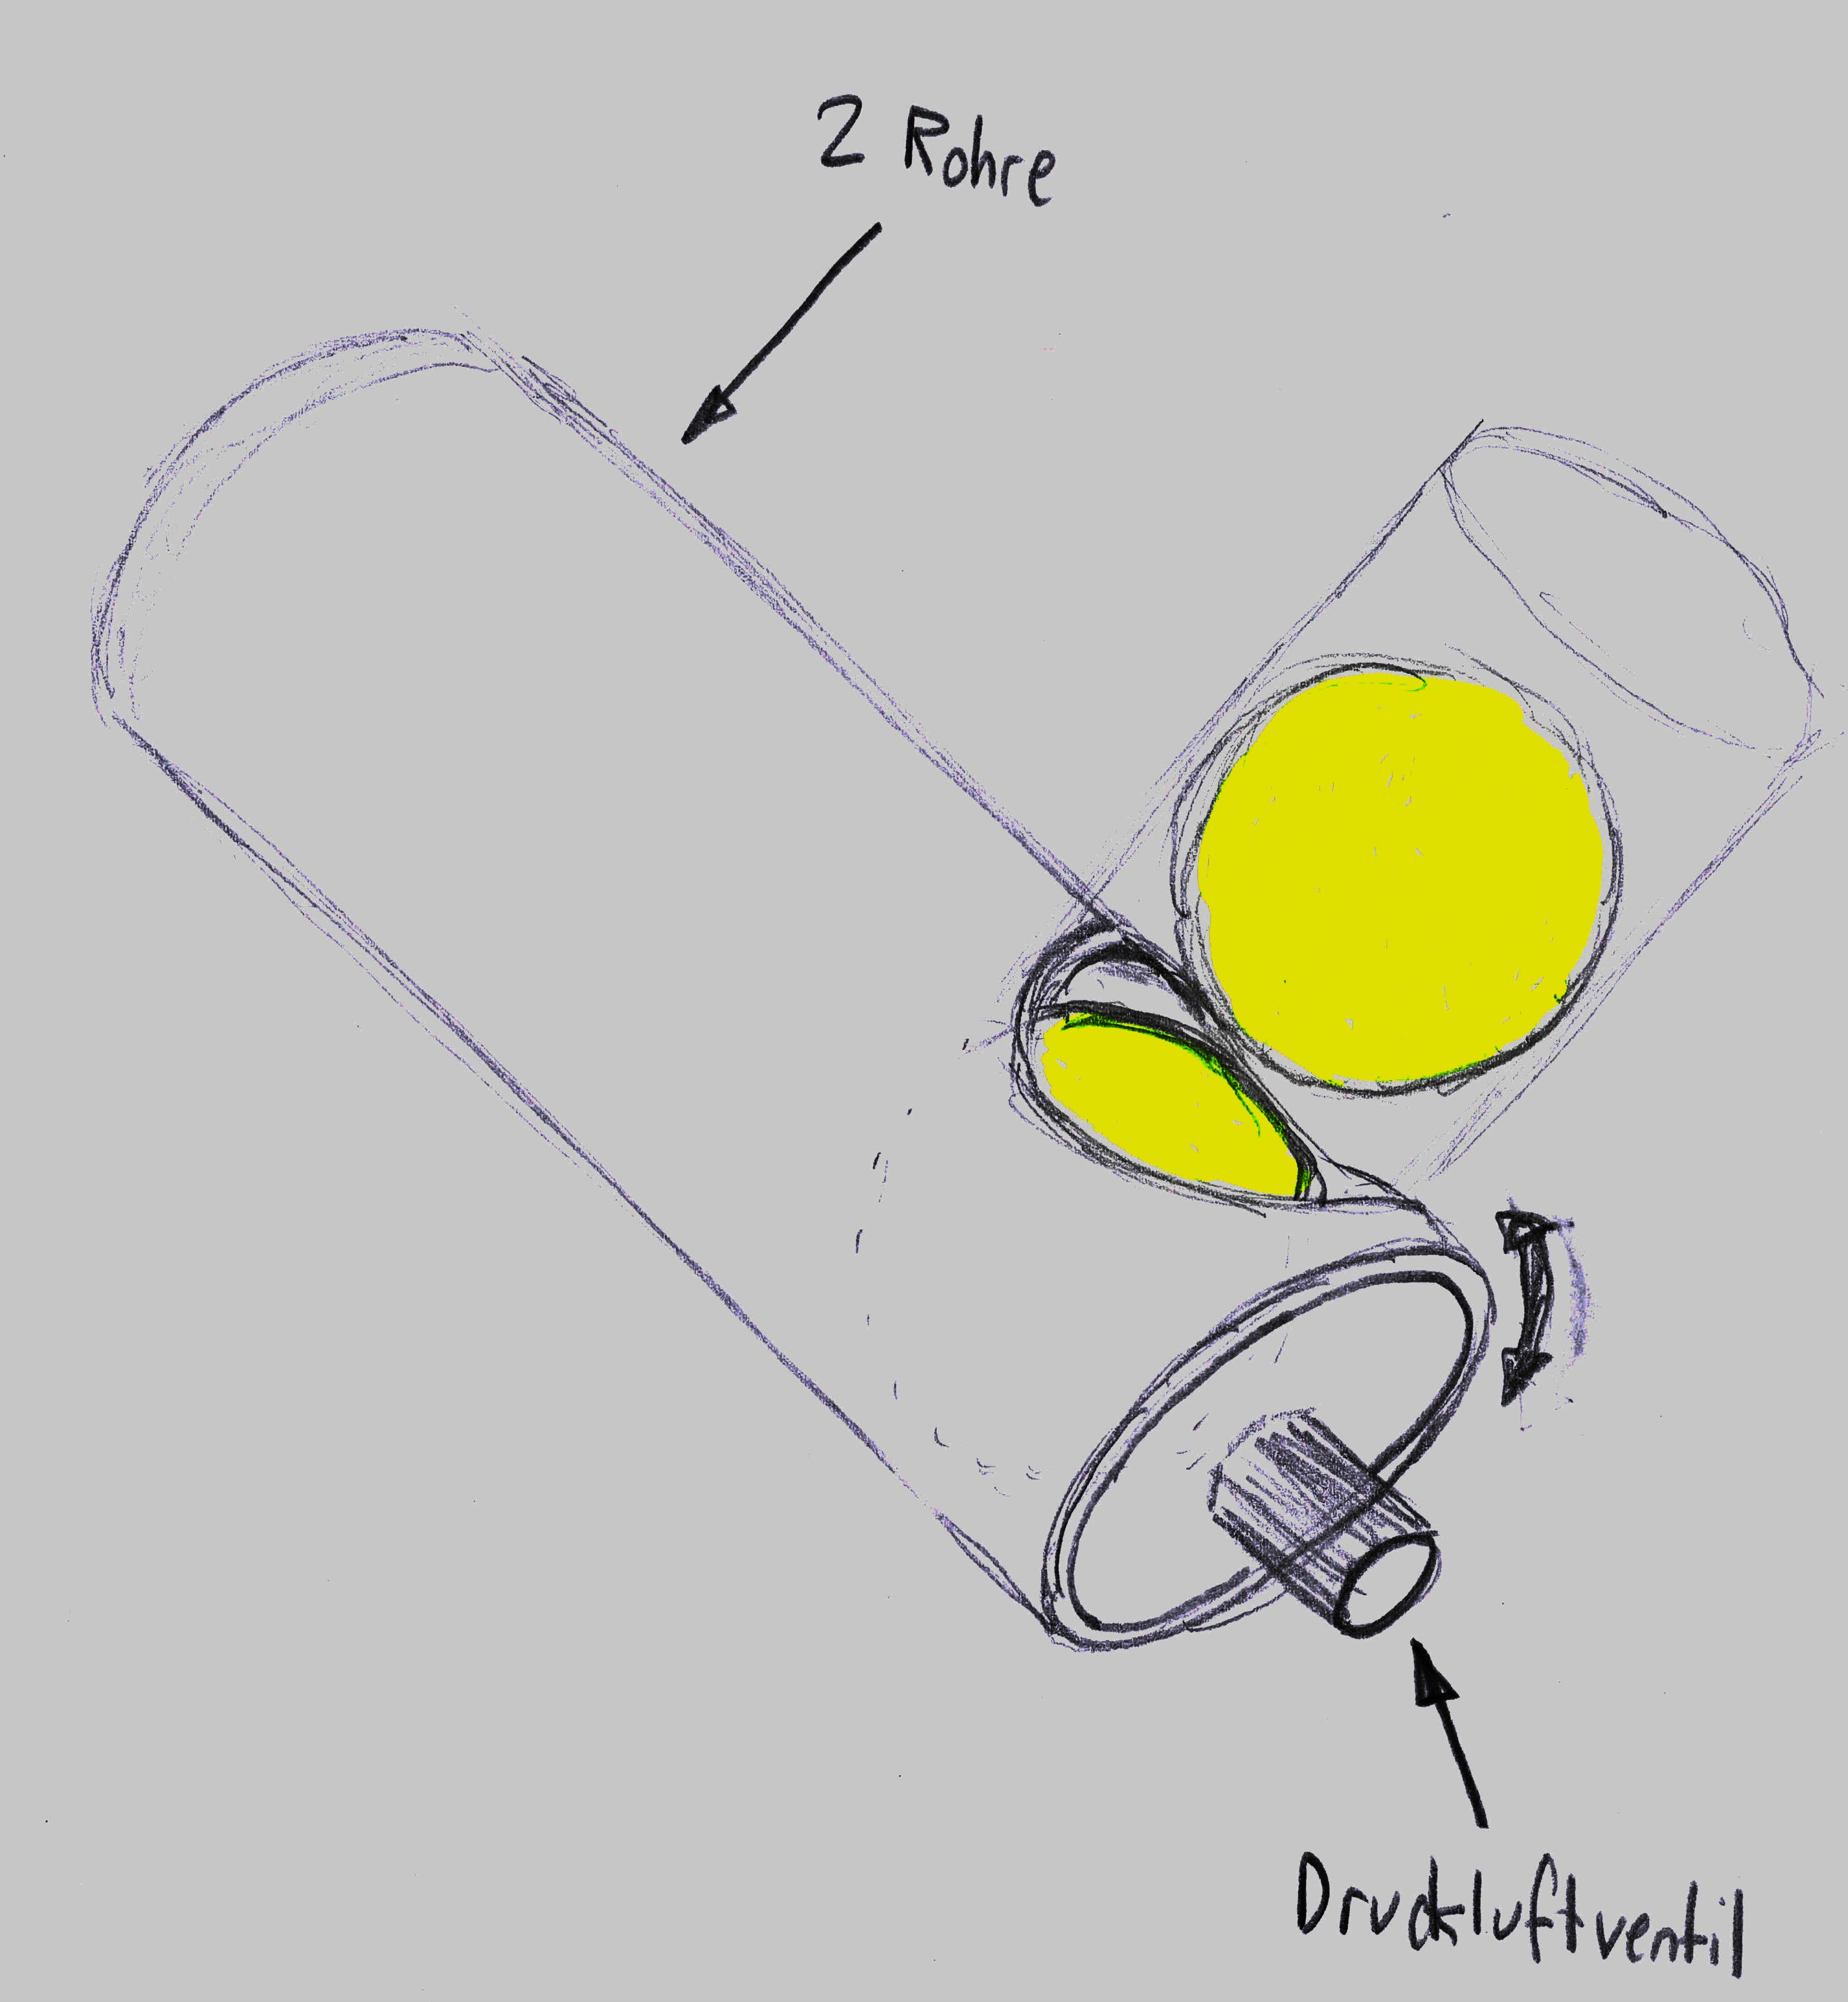
\includegraphics[width=0.4\textwidth]{../../fig/Druckluftrohr.jpg}
	\caption{Druckluftrohr}
	\label{fig:druckluftrohr}
\end{figure}
\subsection{Idee}
Die Idee ist Druckluft zu benutzen, um ein Ball aufs mal durch ein Rohr zu beschleunigen. Es wird der zur verfügung stehende Druckluftsanschluss benutzt. Da die Bälle einen Durchmesserdifferenz bis zu 1 cm haben können, kann der Rohr nicht Dicht sein. Aus diesem Grund werden wir ein Rohr benutzen der ein Durchmesser nur wenig grösser als das grösste Ball hat und wir werden den Rohr so modifizieren, dass gerade nach die Aufladungszone enger ist so dass alle Bälle dort sich blockieren. Dank diese Verengerung blockiert sich den Ball und die Luftdruck hinter der Ball wird immer grösser, bis es genug ist um der Ball durch die Verengerung ausdrucken. Dieses Prozess wird am Ball genugend Energie geben um bis zum Korb zu fliegen.
Die Nachladung der Bälle kann mit einem zweiten Rohr gemacht werden, der sich um der erste Rohr dreht. Diese Röhre sind beide so geschnitten, dass wenn die beide Schnitte übereinstimmen ein neuer Ball im ersten Rohr fallt. Wenn die beide Schnitte nicht übereinstimmen ist der erste Rohr dicht.
\subsection{Annahmen}
Um sicherzustellen, dass das Konzept funktioniert, mussen die Schrumpfung und der Ball eng anliegend, so dass die Druckluft genügend Druck um den Ball schießen erstellen kann. Deswegen darf der Durchmesser der Bälle nicht zu unterschiedlich sein. 

\subsection{Risiken}
Falls der Durchmesser der Bälle zu unterschiedlich ist, kann bei einigen passieren, dass sie nicht der Korb treffen weil der Druck nicht genügend oder zu gross war. Weil der Rohr etwas grösser als die Bälle ist, gibt es die Möglichkeit, dass die Bälle bei dem Wurf links oder rechts biegen oder sogar einklemmen.

\subsection{Bewertung}
